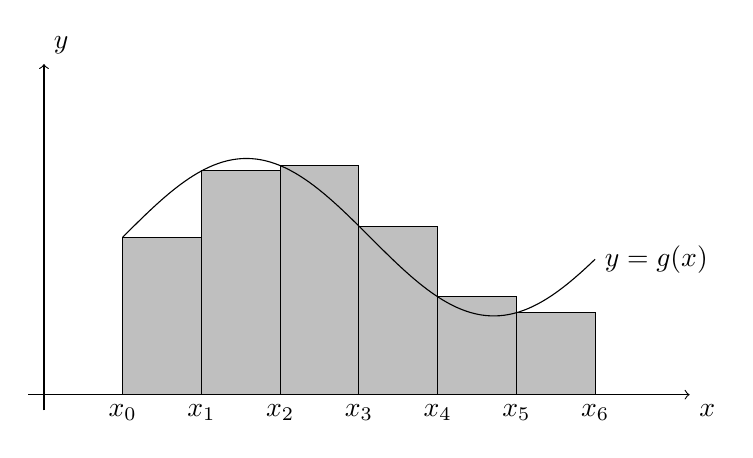
\begin{tikzpicture}
  \draw[->] (-.2,0) -- (8.2,0) node[below right] {$x$};
  \draw[->] (0,-.2) -- (0,4.2) node[above right] {$y$};

  \foreach \x in {0,1,...,5} {%
    \draw[fill=gray!50] (\x + 1,0) -- ++(1,0) -- ++(0,{sin(\x r) ++ 2}) --
    ++(-1,0) -- ++(0,{-sin(\x r) - 2});
  }

  \draw[domain=0:6,samples=100] plot(\x + 1,{sin(\x r) + 2})
  node[right] {$y = g(x)$};

  \foreach \x in {0,1,...,6} {%
    \draw (\x + 1,0) node[below] {$x_{\x}$};
  }
\end{tikzpicture}
